\chapter{編輯環境} \label{ch_enviornment}

本章描述使用專案時需要環境設定。本章節分為作業系統說明、CLI 以及 Docker。
NKUST-latex-template 編譯環境僅需由 CLI 和 Docker 之中擇一即可。
本專案僅需要基礎的文字編輯器 vi、emase、notepad 等搭配 command line 即可使用,但我們推薦使用 VSCode 進行編輯,能讓您有較舒適的整合性使用體驗。

\section{Windows環境說明}

本節是針對 Windows 使用者的說明,UNIX-like 作業系統使用者請略過本節,直接跳至 CLI 或 Docker 閱讀。

開發時實驗室皆以 Linux 作業系統為基底進行論文編寫,並沒有 Windows 的開發需求,因此本專案僅使用 bash 的命令進行 makefile 的撰寫,這也是沒有支援原生 windows 命令提示字元的原因。
目前在 Windows 下有 Windows subsystem on Linux (WSL)、Git Bash、Cygwin 等 Bash 相容環境可以使用,下面將列舉這些方案並說明本專案在這些環境上已知的事項。

\subsection{Windows subsystem on Linux}

這是由 Microsoft 開發的作業系統相容層,能夠執行原生的 Linux application,本專案 makefile 中使用的指令都可以使用。
CLI 方案的使用者可以選擇將 texlive 安裝在 windows 中或是由 WSL 的 Linux 套件管理員進行安裝即可使用。

2021 年 08 月 31 日,Docker 更改了 Docker Desktop 的使用規則,超過 250 人的單位需要支付費用,但教育版本及私人使用維持免費授權。
目前這個專案只需使用 Docker Engine 與 CLI,沒有 Desktop GUI 依然能正常使用。
因此如果您為在學學生,但住宿區域的網域必需迴避此規定時,請在 WSL2 的 Linux 上安裝 Docker 即可,並由 WSL2 執行 Docker 撰寫論文。

\subsection{Git Bash}

CLI 方案理論上可遷移至 Git Bash 上執行,但 Windows 需安裝 TexLive 工具鏈。
Docker 方案使用者應可直接使用,但與 CLI 方案相同需先在 Windows 中安裝 Docker。此環境我們沒有進行過相關測試,效率與執行時期會發生的情況未知,趕時間的話不建議使用。

\subsection{Cygwin}

此功能未經過驗證,使用者必須自行安裝各式各樣的相依套件,不建議使用。

\section{CLI}

CLI 操作環境依賴 bash 等 UNIX-like 的環境,僅需要安裝 TexLive 與 Make 即可使用使用基礎的文字編輯器與 command line 編寫論文。

\section{Docker}

本節紀錄使用 Docker 快速佈署論文編譯環境的操作流程。在閱讀前請先注意以下注意事項。

\begin{itemize}
        \item 本專案的論文主體請存放於 host\footnote{附註:Host 系統指的是您 Docker 安裝的基底系統,正常情況下是 Windows、Linux 或是 MacOS,如果 Docker 是安裝於 WSL2 中,這個 Host 指的是 WSL2。} 系統中,Docker image 啟動時會自動將您的論文目錄掛載到 container 中。
        \item 當 container 被關閉時,除論文目錄以外的 container 的資料都會被抹除。如要有須保留 container 資料請在 \emph{docker run} 的啟動參數中移除 $--$rm 即可。
\end{itemize}

Docker 安裝請參閱官方文件。

\begin{itemize}
        \item Windows\cite{win_docker}
        \item Linux\cite{linux_docker}
        \item MacOS\cite{mac_docker}
\end{itemize}

\subsection{Bash}

本節適用於 Docker 安裝於 Linux、MacOS、WSL 中的使用者。

編譯 docker image,客制化使用者開發環境參數,基底源自 texlive\cite{docker_texlive}。
\begin{lstlisting}[language=bash]
        $ ./Docker/linux/build
\end{lstlisting}

啟動 latex-srv,使用腳本會運作於背景中。

\begin{lstlisting}[language=bash]
        $ ./Docker/linux/start
\end{lstlisting}

如須進入到環境的 \emph{bash} 中,可以透過 attach 進入環境。如果要離開環境請用 \emph{Ctrl-P} + \emph{Ctrl-Q},如使用 exit 將會關閉該 container。
\begin{lstlisting}[language=bash] 
        $ ./Docker/linux/attach
\end{lstlisting}

關閉 latex-srv,關閉運作於背景的 container。除了這個指令可以關閉 container 外,也可以在 container 中執行 exit 來關閉 container。
\begin{lstlisting}[language=bash]
        $ ./Docker/linux/stop
\end{lstlisting}

\newpage

\subsection{CMD / PowerShell}

本節適用於已於 Windows 中安裝 Docker Desktop 的使用者。

編譯 docker image,客制化使用者開發環境參數,基底源自 texlive\cite{docker_texlive},可使用滑鼠雙擊 \emph{build.bat} 或使用 \emph{cmd} / \emph{powershell} 執行。
\begin{lstlisting}[language=bash]
        > ./Docker/windows/build.bat
\end{lstlisting}

啟動 latex-srv,使用腳本會運作於背景中,可使用滑鼠雙擊 \emph{build.bat} 或使用 cmd / powershell 執行。
\begin{lstlisting}[language=bash]
        > ./Docker/windows/start.bat
\end{lstlisting}

如須進入到環境的 \emph{bash} 中,可以透過 attach 進入環境。如果要離開環境請用 \emph{Ctrl-P} + \emph{Ctrl-Q},如使用 exit 將會關閉該 container,可使用滑鼠雙擊 build.bat 或使用 cmd / powershell 執行。
\begin{lstlisting}[language=bash]
        > ./Docker/windows/attach.bat
\end{lstlisting}

關閉 latex-srv,關閉運作於背景的 container,可使用滑鼠雙擊 \emph{build.bat} 或使用 \emph{cmd} / \emph{powershell} 執行。
\begin{lstlisting}[language=bash]
        > ./Docker/windows/stop.bat
\end{lstlisting}

\newpage

\subsection{Docker 方案中使用 VSCode 編輯}

透過 vscode remote extension 進行連線操作,支援 Docker 目錄中所有工具。

\subsubsection*{步驟一}
編譯 image,可雙擊檔案或以 terminal 於專案目錄中執行編譯指令,在此之前請安裝完 docker。如果發生 Image 中已有與您相同名稱使用者,請直接修改 build 來指定 USER / USERID 等資訊。務必注意,修改使用者資訊意味著您在非 docker 的環境中時,檔案會有操作權限的問題。

\begin{flushleft}
        \textbf{Linux、MacOS、WSL}
\end{flushleft}

\begin{lstlisting}[language=bash]
        $ ./Docker/linux/build
\end{lstlisting}

\begin{flushleft}
        \textbf{Windows}
\end{flushleft}

\begin{lstlisting}[language=bash]
        > ./Docker/windows/build.bat
\end{lstlisting}

\subsubsection*{步驟二}

安裝 remote extension,如圖\ref{fig_vscode_remote_extension}。

\begin{figure}[H] 
        \centering 
        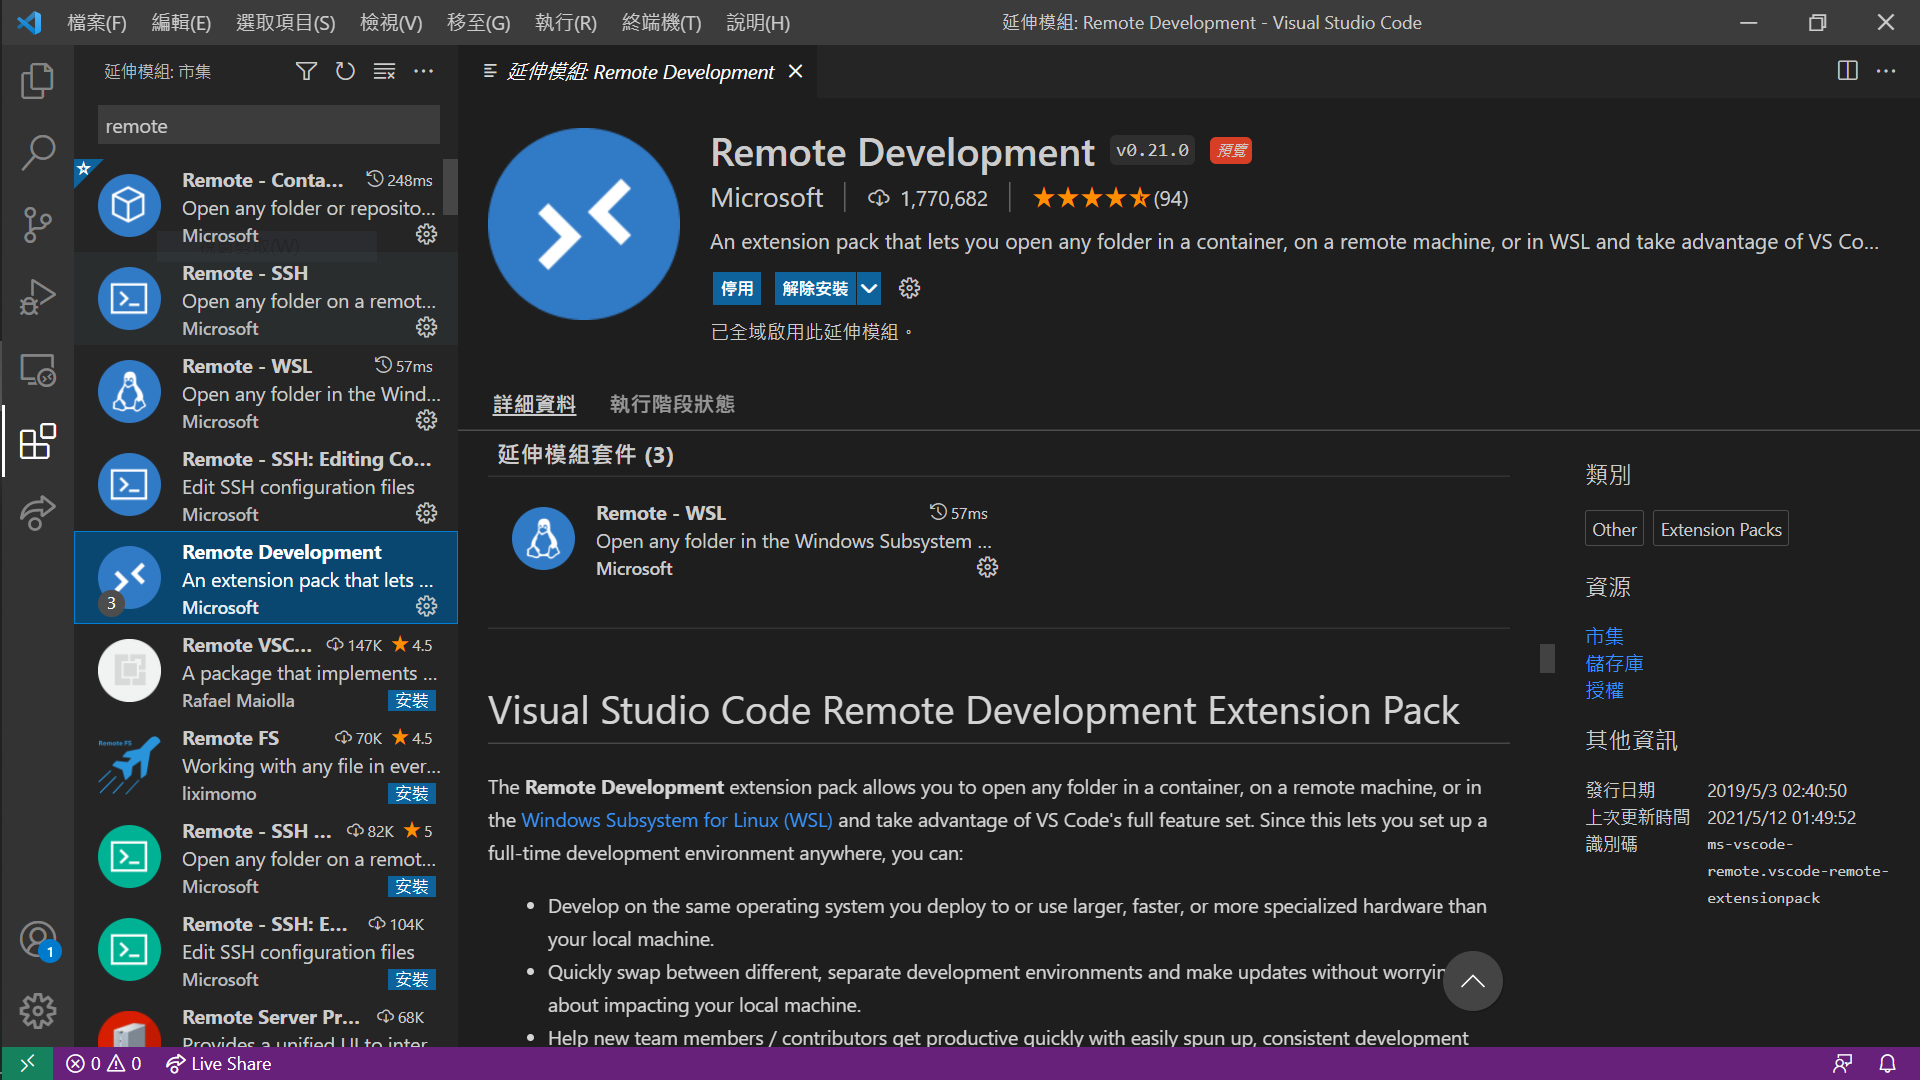
\includegraphics[width=0.8\textwidth]{./Figures/Env/docker/vscode_remote_extension.png} 
        \caption{安裝 remote extension}
        \label{fig_vscode_remote_extension}
\end{figure}

\subsubsection*{步驟三}

啟動 container 進行服務可雙擊檔案或以 terminal 於專案目錄中執行啟動指令。如果正常運作執行後終端機將會自動關閉。

\begin{flushleft}
        \textbf{Linux、MacOS、WSL}
\end{flushleft}

\begin{lstlisting}[language=bash]
        $ ./Docker/linux/start
\end{lstlisting}

\begin{flushleft}
        \textbf{Windows}
\end{flushleft}

\begin{lstlisting}[language=bash]
        > ./Docker/windows/start.bat
\end{lstlisting}

\subsubsection*{步驟四}

Ctrl-P 呼叫命令工具,找到(可直接輸入) \emph{> Remote-Container: Attach to Running container ...},如圖\ref{fig_vscode_select_container},點擊後選擇 latex-srv 即可進入開發環境,如圖\ref{fig_vscode_attach_container}。

\begin{figure}[H] 
        \centering 
        \subfigure{
                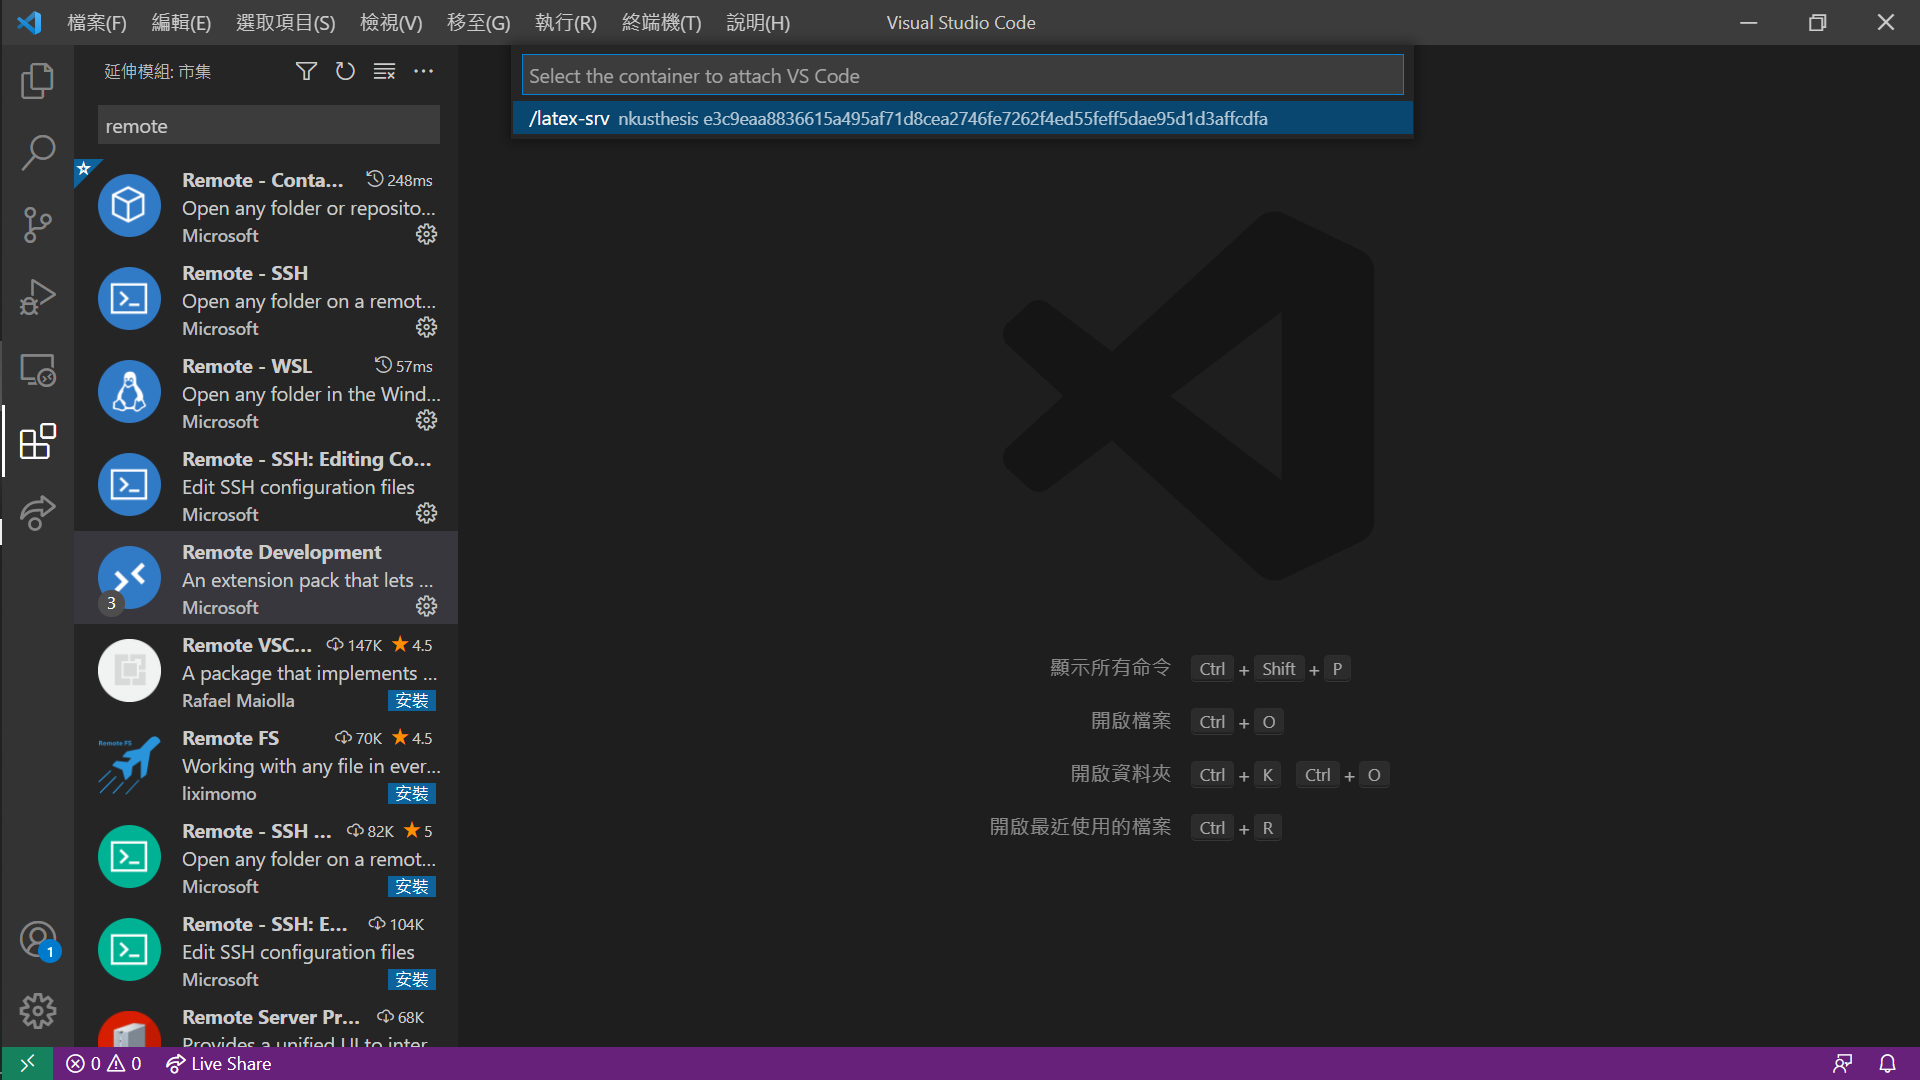
\includegraphics[width=0.8\textwidth]{./Figures/Env/docker/vscode_select_container.png}
                \label{fig_vscode_select_container}
        }
        \quad
        \centering 
        \subfigure{
                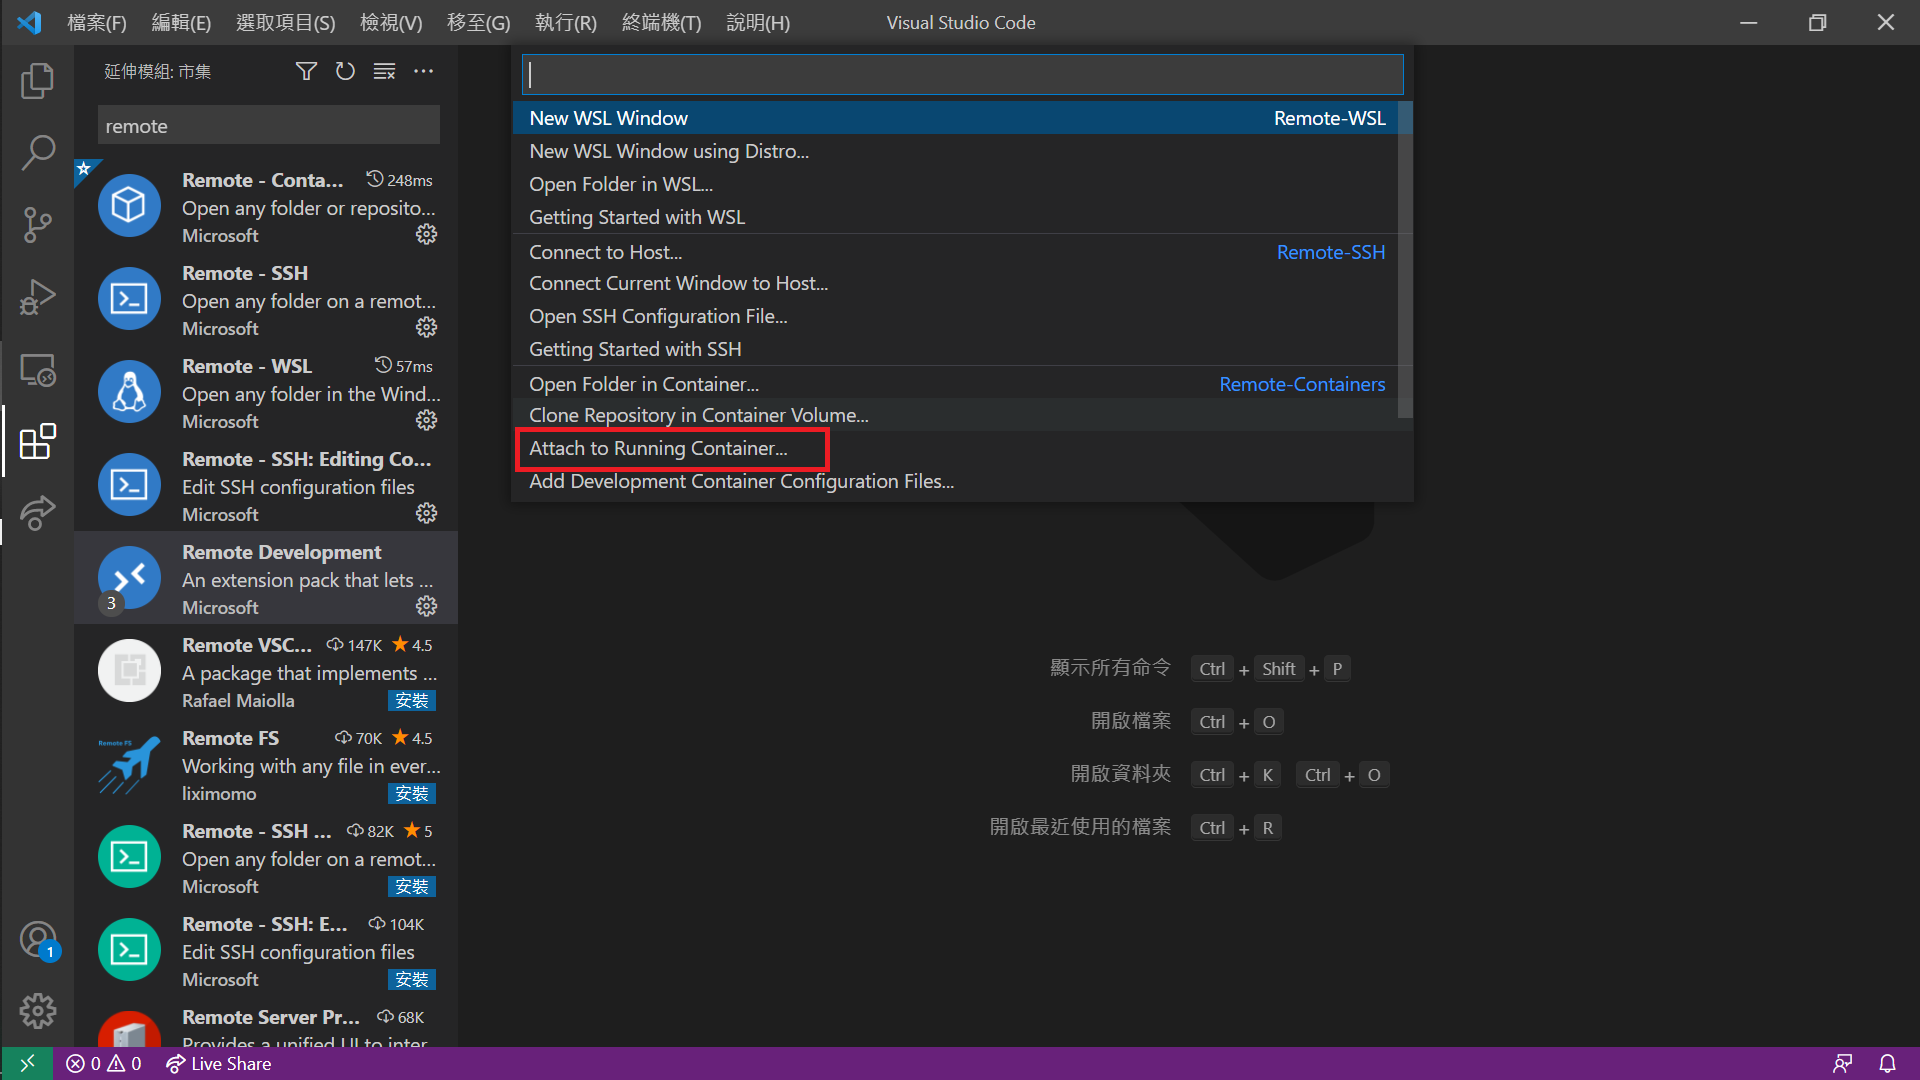
\includegraphics[width=0.8\textwidth]{./Figures/Env/docker/vscode_attach_container.png}
                \label{fig_vscode_attach_container}
        }
        \caption{Attach to Running container}
\end{figure}

\subsubsection*{步驟五}

開啟資料夾,論文目錄預設掛載在 \emph{/home/<username>/thesis} 中,如圖\ref{fig_vscode_finish}。

\begin{figure}[H] 
        \centering 
        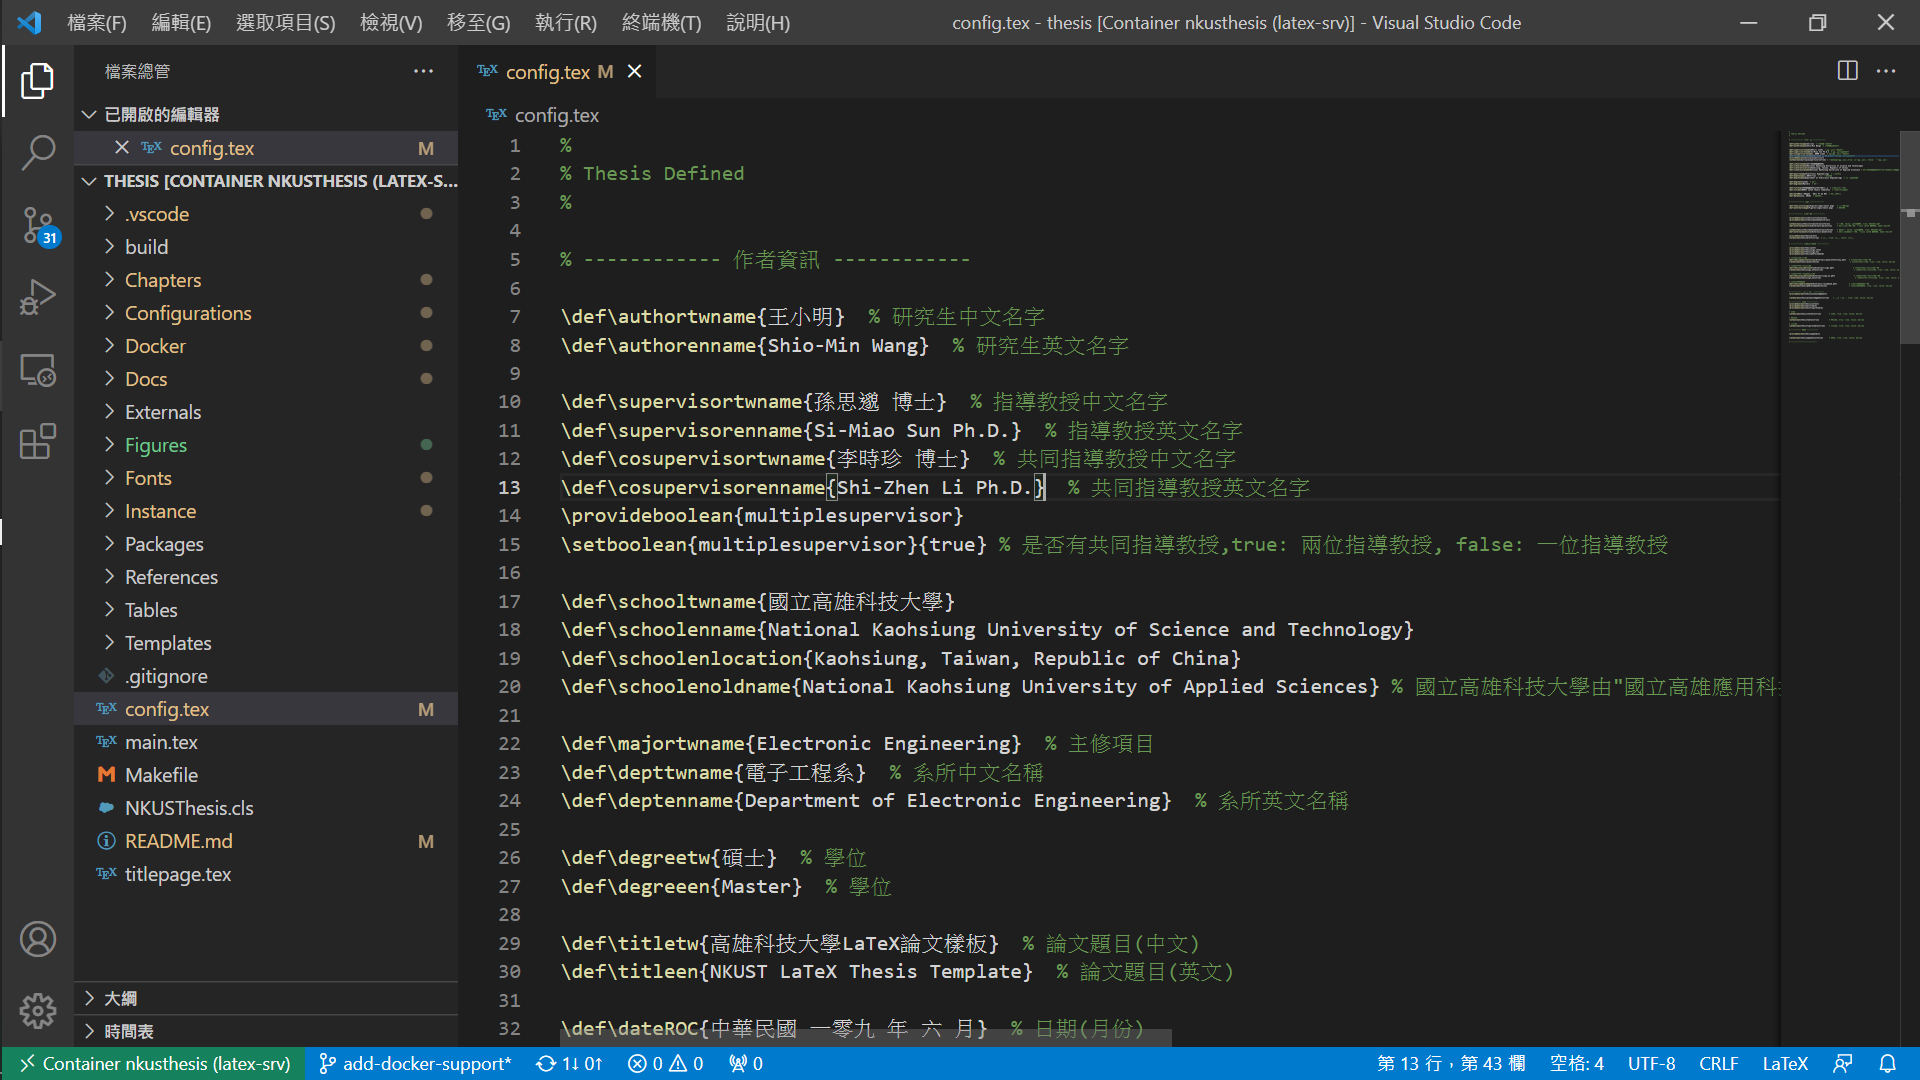
\includegraphics[width=0.8\textwidth]{./Figures/Env/docker/vscode_finish.png} 
        \caption{完成開啟 Container 中的論文目錄}
        \label{fig_vscode_finish}
\end{figure}
